\chapter{Matrius}

\index{matriu}

Una \key{matriu} és un concepte matemàtic que es correspon amb una taula
bidimensional en programació. Per exemple,
\[
A = 
 \begin{bmatrix}
  6 & 13 & 7 & 4 \\
  7 & 0 & 8 & 2 \\
  9 & 5 & 4 & 18 \\
 \end{bmatrix}
\]
és una matriu de mida $3 \times 4$, és a dir, té 3 files i 4
columnes. La notació $[i,j]$ fa referència a l'element de la fila $i$
i la columna $j$ d'una matriu. Per exemple, a la matriu anterior,
$A[2,3]=8$ i $A[3,1]=9$.

\index{vector}

Un cas especial d'una matriu és un \key{vector} que és una matriu
unidimensional de mida $n \times 1$. Per exemple,
\[
V =
\begin{bmatrix}
4 \\
7 \\
5 \\
\end{bmatrix}
\]
és un vector que conté tres elements.

\index{transposta}

La \key{matriu transposta} $A^T$ d'una matriu $A$ s'obté quan s'intercanvien
les files i columnes de $A$, és a dir, $A^T[i,j]=A[j,i]$:
\[
A^T = 
 \begin{bmatrix}
  6 & 7 & 9 \\
  13 & 0 & 5 \\
  7 & 8 & 4 \\
  4 & 2 & 18 \\
 \end{bmatrix}
\]


\index{matriu quadrada}

Una matriu és una \key{matriu quadrada} si té el mateix nombre de
files i columnes. Per exemple, la matriu següent és una matriu
quadrada:


\[
S = 
 \begin{bmatrix}
  3 & 12 & 4  \\
  5 & 9 & 15  \\
  0 & 2 & 4 \\
 \end{bmatrix}
\]


\section{Operacions}

La suma $A+B$ de les matrius $A$ i $B$ només es defineix quan les
matrius són de la mateixa mida. El resultat és una matriu on cada
element és la suma dels elements corresponents en $A$ i $B$.

Per exemple,
\[
 \begin{bmatrix}
  6 & 1 & 4 \\
  3 & 9 & 2 \\
 \end{bmatrix}
+
 \begin{bmatrix}
  4 & 9 & 3 \\
  8 & 1 & 3 \\
 \end{bmatrix}
=
 \begin{bmatrix}
  6+4 & 1+9 & 4+3 \\
  3+8 & 9+1 & 2+3 \\
 \end{bmatrix}
=
 \begin{bmatrix}
  10 & 10 & 7 \\
  11 & 10 & 5 \\
 \end{bmatrix}.
\]


Multiplicar una matriu $A$ per un valor $x$ dóna una matriu $xA$ on
cada element de $A$ es multiplica per $x$. Per exemple,
\[
 2 \cdot \begin{bmatrix}
  6 & 1 & 4 \\
  3 & 9 & 2 \\
 \end{bmatrix}
=
 \begin{bmatrix}
  2 \cdot 6 & 2\cdot1 & 2\cdot4 \\
  2\cdot3 & 2\cdot9 & 2\cdot2 \\
 \end{bmatrix}
=
 \begin{bmatrix}
  12 & 2 & 8 \\
  6 & 18 & 4 \\
 \end{bmatrix}.
\]


\subsubsection{Multiplicació de matrius}

\index{multiplicació de matrius}

El producte $AB$ de les matrius $A$ i $B$ es defineix si $A$ és de
mida $a \times n$ i $B$ és de mida $n \times b$, és a dir, l'amplada
(mida d'una fila) de $A$ és igual a l'alçada (mida d'una columna) de
$B$. El resultat és una matriu de mida $a \times b$ els elements de la
qual es calculen mitjançant la fórmula
\[
AB[i,j] = \sum_{k=1}^n A[i,k] \cdot B[k,j].
\]


La idea és que cada element de $AB$ és la suma de productes dels
elements de $A$ i $B$ segons la imatge següent:


\begin{center}
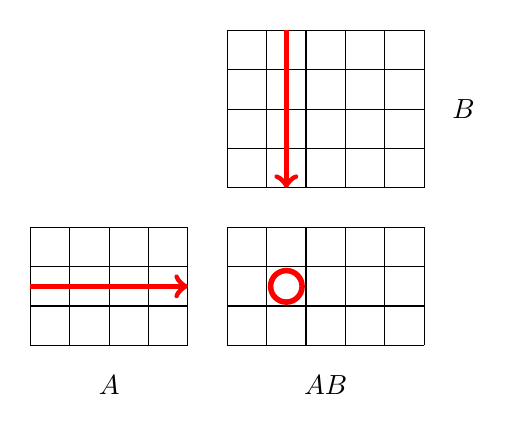
\begin{tikzpicture}[scale=0.5]
\draw (0,0) grid (4,3);
\draw (5,0) grid (10,3);
\draw (5,4) grid (10,8);

\node at (2,-1) {$A$};
\node at (7.5,-1) {$AB$};
\node at (11,6) {$B$};

\draw[thick,->,red,line width=2pt] (0,1.5) -- (4,1.5);
\draw[thick,->,red,line width=2pt] (6.5,8) -- (6.5,4);
\draw[thick,red,line width=2pt] (6.5,1.5) circle (0.4);
\end{tikzpicture}
\end{center}


Per exemple,


\[
 \begin{bmatrix}
  1 & 4 \\
  3 & 9 \\
  8 & 6 \\
 \end{bmatrix}
\cdot
 \begin{bmatrix}
  1 & 6 \\
  2 & 9 \\
 \end{bmatrix}
=
 \begin{bmatrix}
  1 \cdot 1 + 4 \cdot 2 & 1 \cdot 6 + 4 \cdot 9 \\
  3 \cdot 1 + 9 \cdot 2 & 3 \cdot 6 + 9 \cdot 9 \\
  8 \cdot 1 + 6 \cdot 2 & 8 \cdot 6 + 6 \cdot 9 \\
 \end{bmatrix}
=
 \begin{bmatrix}
  9 & 42 \\
  21 & 99 \\
  20 & 102 \\
 \end{bmatrix}.
\]


La multiplicació de matrius és associativa, i per tant es compleix $A(BC)=(AB)C$,
però no és commutativa, de manera que, en general, no es compleix que $AB = BA$.

\index{matriu identitat}

La \key{matriu identitat} de mida $n$ és una matriu quadrada on cada element de la
diagonal és 1 i tots els altres elements són 0. Per exemple, la matriu
següent és la matriu identitat de mida $3$:

\[
 I = \begin{bmatrix}
  1 & 0 & 0 \\
  0 & 1 & 0 \\
  0 & 0 & 1 \\
 \end{bmatrix}
\]


Multiplicar una matriu per la matriu identitat és el mateix que no fer res.
Per exemple,
\[
 \begin{bmatrix}
  1 & 0 & 0 \\
  0 & 1 & 0 \\
  0 & 0 & 1 \\
 \end{bmatrix}
\cdot
 \begin{bmatrix}
  1 & 4 \\
  3 & 9 \\
  8 & 6 \\
 \end{bmatrix}
=
 \begin{bmatrix}
  1 & 4 \\
  3 & 9 \\
  8 & 6 \\
 \end{bmatrix} \hspace{10px} \textrm{and} \hspace{10px}
 \begin{bmatrix}
  1 & 4 \\
  3 & 9 \\
  8 & 6 \\
 \end{bmatrix}
\cdot
 \begin{bmatrix}
  1 & 0 \\
  0 & 1 \\
 \end{bmatrix}
=
 \begin{bmatrix}
  1 & 4 \\
  3 & 9 \\
  8 & 6 \\
 \end{bmatrix}.
\]


Fent servir un algorisme senzill, podem calcular el producte de dues
matrius $n \times n$ en temps $O(n^3)$. També hi ha algorismes més
eficients per a la multiplicació de matrius\footnote{El primer
algorisme d'aquest tipus va ser l'algorisme de Strassen, publicat el
1969 \cite{str69}, la complexitat temporal del qual és
$O(n^{2.80735})$; el millor algorisme actual \cite{gal14} funciona en
temps $O(n^{2.37286})$.}, però són sobretot d'interès teòric i aquests
algorismes no són necessaris en la programació competitiva.



\subsubsection{Potència d'una matriu}

\index{potència d'una matriu}

La potència $A^k$ d'una matriu $A$ es defineix si $A$ és una matriu
quadrada. La definició es basa en la multiplicació de matrius:
\[ A^k = \underbrace{A \cdot A \cdot A \cdots A}_{\textrm{$k$ times}} \]
Per exemple,


\[
 \begin{bmatrix}
  2 & 5 \\
  1 & 4 \\
 \end{bmatrix}^3 =
 \begin{bmatrix}
  2 & 5 \\
  1 & 4 \\
 \end{bmatrix} \cdot
 \begin{bmatrix}
  2 & 5 \\
  1 & 4 \\
 \end{bmatrix} \cdot
 \begin{bmatrix}
  2 & 5 \\
  1 & 4 \\
 \end{bmatrix} =
 \begin{bmatrix}
  48 & 165 \\
  33 & 114 \\
 \end{bmatrix}.
\]
A més, $A^0$ és la matriu identitat. Per exemple,
\[
 \begin{bmatrix}
  2 & 5 \\
  1 & 4 \\
 \end{bmatrix}^0 =
 \begin{bmatrix}
  1 & 0 \\
  0 & 1 \\
 \end{bmatrix}.
\]


La matriu $A^k$ es pot calcular eficientment en temps $O(n^3 \log k)$
usant l'algorisme del capítol 21.2. Per exemple,
\[
 \begin{bmatrix}
  2 & 5 \\
  1 & 4 \\
 \end{bmatrix}^8 =
 \begin{bmatrix}
  2 & 5 \\
  1 & 4 \\
 \end{bmatrix}^4 \cdot
 \begin{bmatrix}
  2 & 5 \\
  1 & 4 \\
 \end{bmatrix}^4.
\]


\subsubsection{Determinant}

\index{determinant}

El \key{determinant} $\det(A)$ d'una matriu $A$ es defineix si $A$ és
una matriu quadrada. Si $A$ és de mida $1 \times 1$, llavors
$\det(A)=A[1,1]$. El determinant d'una matriu més gran es calcula
recursivament mitjançant la fórmula \index{cofactor}
\[\det(A)=\sum_{j=1}^n A[1,j] C[1,j],\]
on $C[i,j]$ és el \key{cofactor} de $A$ a $[i,j]$. El cofactor es calcula mitjançant la fórmula
\[C[i,j] = (-1)^{i+j} \det(M[i,j]),\]
on $M[i,j]$ s'obté eliminant la fila $i$ i la columna $j$ de $A$. A
causa del coeficient $(-1)^{i+j}$ del cofactor, tots els altres
determinants són positius i negatius. Per exemple,
\[
\det(
 \begin{bmatrix}
  3 & 4 \\
  1 & 6 \\
 \end{bmatrix}
) = 3 \cdot 6 - 4 \cdot 1 = 14 
\]
i
\[
\det(
 \begin{bmatrix}
  2 & 4 & 3 \\
  5 & 1 & 6 \\
  7 & 2 & 4 \\
 \end{bmatrix}
) = 
2 \cdot
\det(
 \begin{bmatrix}
  1 & 6 \\
  2 & 4 \\
 \end{bmatrix}
)
-4 \cdot
\det(
 \begin{bmatrix}
  5 & 6 \\
  7 & 4 \\
 \end{bmatrix}
)
+3 \cdot
\det(
 \begin{bmatrix}
  5 & 1 \\
  7 & 2 \\
 \end{bmatrix}
) = 81.
\]


\index{matriu inversa}

El determinant de $A$ ens indica si hi ha una \key{matriu inversa}
$A^{-1}$ tal que $A \cdot A^{-1} = I$, on $I$ és la matriu
identitat. Resulta que $A^{-1}$ existeix exactament quan $\det(A)
\neq 0$, i es pot calcular mitjançant la fórmula


\[A^{-1}[i,j] = \frac{C[j,i]}{det(A)}.\]


Per exemple,


\[
\underbrace{
 \begin{bmatrix}
  2 & 4 & 3\\
  5 & 1 & 6\\
  7 & 2 & 4\\
 \end{bmatrix}
}_{A}
\cdot
\underbrace{
 \frac{1}{81}
 \begin{bmatrix}
   -8 & -10 & 21 \\
   22 & -13 & 3 \\
   3 & 24 & -18 \\
 \end{bmatrix}
}_{A^{-1}}
=
\underbrace{
 \begin{bmatrix}
  1 & 0 & 0 \\
  0 & 1 & 0 \\
  0 & 0 & 1 \\
 \end{bmatrix}
}_{I}.
\]


\section{Recurrències lineals}

\index{recurrència lineal}

Una \key{recurrència lineal} és una funció $f(n)$ els valors inicials
de la qual són $f(0),f(1),\ldots,f(k-1)$ i els valors més grans es
calculen recursivament mitjançant la fórmula
\[f(n) = c_1 f(n-1) + c_2 f(n-2) + \ldots + c_k f (n-k),\]

on $c_1,c_2,\ldots,c_k$ són coeficients constants.

La programació dinàmica es pot fer servir per calcular qualsevol valor
de $f(n)$ en temps $O(kn)$ calculant tots els valors de
$f(0),f(1),\ldots,f(n)$ un després un altre. Tanmateix, si $k$ és
petit, és possible calcular $f(n)$ de manera molt més eficient en
temps $O(k^3 \log n)$ fent servir operacions amb matrius.

\subsubsection{Nombres de Fibonacci}

\index{Nombre de Fibonacci}

Un exemple senzill de recurrència lineal és la funció següent que
defineix els nombres de Fibonacci:
\[
\begin{array}{lcl}
f(0) & = & 0 \\
f(1) & = & 1 \\
f(n) & = & f(n-1)+f(n-2) \\
\end{array}
\]
En aquest cas, $k=2$ i $c_1=c_2=1$.

\begin{samepage}
  Per calcular de manera eficient els nombres de Fibonacci,
  representem el Fórmula de Fibonacci com un matriu quadrada $X$ de
  mida $2 \times 2$, on es compleix el següent:
\[ X \cdot
 \begin{bmatrix}
  f(i) \\
  f(i+1) \\
 \end{bmatrix}
=
 \begin{bmatrix}
  f(i+1) \\
  f(i+2) \\
 \end{bmatrix}
 \]
 Així, els valors $f(i)$ i $f(i+1)$ es donen com a ''entrada'' per
 $X$, i $X$ calcula els valors $f(i+1)$ i $f(i+2)$ de sortida.  Resulta
 que aquesta matriu és
\[ X =
 \begin{bmatrix}
  0 & 1 \\
  1 & 1 \\
 \end{bmatrix}.
\]
\end{samepage}
\noindent Per exemple,
\[
 \begin{bmatrix}
  0 & 1 \\
  1 & 1 \\
 \end{bmatrix}
\cdot
 \begin{bmatrix}
  f(5) \\
  f(6) \\
 \end{bmatrix}
=
 \begin{bmatrix}
  0 & 1 \\
  1 & 1 \\
 \end{bmatrix}
\cdot
 \begin{bmatrix}
  5 \\
  8 \\
 \end{bmatrix}
=
 \begin{bmatrix}
  8 \\
  13 \\
 \end{bmatrix}
=
 \begin{bmatrix}
  f(6) \\
  f(7) \\
 \end{bmatrix}.
\]
Així, podem calcular $f(n)$ mitjançant la fórmula
\[
 \begin{bmatrix}
  f(n) \\
  f(n+1) \\
 \end{bmatrix}
=
X^n \cdot
 \begin{bmatrix}
  f(0) \\
  f(1) \\
 \end{bmatrix}
=
 \begin{bmatrix}
  0 & 1 \\
  1 & 1 \\
 \end{bmatrix}^n
\cdot
 \begin{bmatrix}
  0 \\
  1 \\
 \end{bmatrix}.
\]
El valor de $X^n$ es pot calcular en temps $O(\log n)$, de manera que
el valor de $f(n)$ també es pot calcular en temps $O(\log n)$.

\subsubsection{Cas general}

Considerem ara el cas general on $f(n)$ és qualsevol recurrència
lineal. De nou, el nostre objectiu és construir una matriu $X$ per a
la qual
\[ X \cdot \begin{bmatrix} f(i) \\ f(i+1) \\ \vdots \\ f(i+k-1) \\ \end{bmatrix} = \begin{bmatrix} f (i+1) \\ f(i+2) \\ \vdots \\ f(i+k) \\ \end{bmatrix}. \]

Aquesta matriu és
\[
X =
 \begin{bmatrix}
  0 & 1 & 0 & 0 & \cdots & 0 \\
  0 & 0 & 1 & 0 & \cdots & 0 \\
  0 & 0 & 0 & 1 & \cdots & 0 \\
  \vdots & \vdots & \vdots & \vdots & \ddots & \vdots \\
  0 & 0 & 0 & 0 & \cdots & 1 \\
  c_k & c_{k-1} & c_{k-2} & c_{k-3} & \cdots & c_1 \\
 \end{bmatrix}.
\]
A les primeres $k-1$ files, cada element és 0, excepte per a un
element que és 1. Aquestes files substitueixen $f(i)$ per $f(i+1)$,
$f(i+1)$ per $ f(i+2)$, i així successivament. L'última fila conté els
coeficients de la recurrència per calcular el nou valor $f(i+k)$.

Ara, $f(n)$ es pot calcular en temps $O(k^3 \log n)$ fent servir la fórmula
\[
 \begin{bmatrix}
  f(n) \\
  f(n+1) \\
  \vdots \\
  f(n+k-1) \\
 \end{bmatrix}
=
X^n \cdot
 \begin{bmatrix}
  f(0) \\
  f(1) \\
  \vdots \\
  f(k-1) \\
 \end{bmatrix}.
\]


\section{Grafs i matrius}

\subsubsection{Comptar camins}

Les potències de la matriu d'adjacència d'un graf tenen una propietat
interessant. Quan $V$ és una matriu d'adjacència en un graf sense
pesos ponderat, la matriu $V^n$ conté el nombre de camins de $n$
arestes entre els nodes del graf.

Per exemple, per al graf
\begin{center}
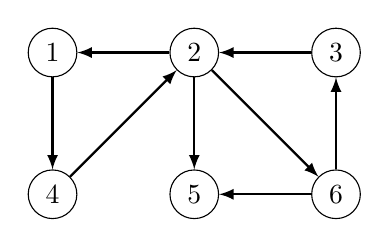
\begin{tikzpicture}[scale=0.9]
\node[draw, circle] (1) at (1,3) {$1$};
\node[draw, circle] (2) at (1,1) {$4$};
\node[draw, circle] (3) at (3,3) {$2$};
\node[draw, circle] (4) at (5,3) {$3$};
\node[draw, circle] (5) at (3,1) {$5$};
\node[draw, circle] (6) at (5,1) {$6$};

\path[draw,thick,->,>=latex] (1) -- (2);
\path[draw,thick,->,>=latex] (2) -- (3);
\path[draw,thick,->,>=latex] (3) -- (1);
\path[draw,thick,->,>=latex] (4) -- (3);
\path[draw,thick,->,>=latex] (3) -- (5);
\path[draw,thick,->,>=latex] (3) -- (6);
\path[draw,thick,->,>=latex] (6) -- (4);
\path[draw,thick,->,>=latex] (6) -- (5);
\end{tikzpicture}
\end{center}
la matriu d'adjacència és
\[
V= \begin{bmatrix}
  0 & 0 & 0 & 1 & 0 & 0 \\
  1 & 0 & 0 & 0 & 1 & 1 \\
  0 & 1 & 0 & 0 & 0 & 0 \\
  0 & 1 & 0 & 0 & 0 & 0 \\
  0 & 0 & 0 & 0 & 0 & 0 \\
  0 & 0 & 1 & 0 & 1 & 0 \\
 \end{bmatrix}.
\]
Ara, per exemple, la matriu
\[
V^4= \begin{bmatrix}
  0 & 0 & 1 & 1 & 1 & 0 \\
  2 & 0 & 0 & 0 & 2 & 2 \\
  0 & 2 & 0 & 0 & 0 & 0 \\
  0 & 2 & 0 & 0 & 0 & 0 \\
  0 & 0 & 0 & 0 & 0 & 0 \\
  0 & 0 & 1 & 1 & 1 & 0 \\
 \end{bmatrix}
\]
conté el nombre de camins de 4 arestes entre els nodes. Per exemple,
$V^4[2,5]=2$, perquè hi ha dos camins de 4 arestes des del node 2 fins
al node 5: $2 \rightarrow 1 \rightarrow 4 \rightarrow 2 \rightarrow 5$
i $2 \rightarrow 6 \rightarrow 3 \rightarrow 2 \rightarrow 5$.

\subsubsection{Camins més curts}

Fent servir una idea semblant per als grafs amb pesos, podem calcular per a
cada parell de nodes la longitud mínima d'un camí entre ells que conté
exactament $n$ arestes. Per calcular-ho, hem de definir la
multiplicació de matrius d'una manera nova, de manera que no calculem
el nombre de camins sinó que minimitzem les longituds dels camins.

Com a exemple, considereu el graf següent:
\begin{center}
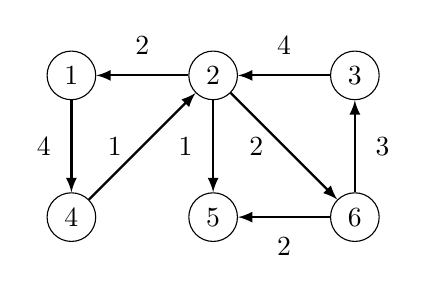
\begin{tikzpicture}[scale=0.9]
\node[draw, circle] (1) at (1,3) {$1$};
\node[draw, circle] (2) at (1,1) {$4$};
\node[draw, circle] (3) at (3,3) {$2$};
\node[draw, circle] (4) at (5,3) {$3$};
\node[draw, circle] (5) at (3,1) {$5$};
\node[draw, circle] (6) at (5,1) {$6$};

\path[draw,thick,->,>=latex] (1) -- node[font=\small,label=left:4] {} (2);
\path[draw,thick,->,>=latex] (2) -- node[font=\small,label=left:1] {} (3);
\path[draw,thick,->,>=latex] (3) -- node[font=\small,label=north:2] {} (1);
\path[draw,thick,->,>=latex] (4) -- node[font=\small,label=north:4] {} (3);
\path[draw,thick,->,>=latex] (3) -- node[font=\small,label=left:1] {} (5);
\path[draw,thick,->,>=latex] (3) -- node[font=\small,label=left:2] {} (6);
\path[draw,thick,->,>=latex] (6) -- node[font=\small,label=right:3] {} (4);
\path[draw,thick,->,>=latex] (6) -- node[font=\small,label=below:2] {} (5);
\end{tikzpicture}
\end{center}


Construïm una matriu d'adjacència on $\infty$ significa que no
existeix cap aresta i els altres valors són els pesos de les
arestes. La matriu és
\[
V= \begin{bmatrix}
  \infty & \infty & \infty & 4 & \infty & \infty \\
  2 & \infty & \infty & \infty & 1 & 2 \\
  \infty & 4 & \infty & \infty & \infty & \infty \\
  \infty & 1 & \infty & \infty & \infty & \infty \\
  \infty & \infty & \infty & \infty & \infty & \infty \\
  \infty & \infty & 3 & \infty & 2 & \infty \\
 \end{bmatrix}.
\]

En lloc de la fórmula
\[
AB[i,j] = \sum_{k=1}^n A[i,k] \cdot B[k,j]
\]
ara fem servir la fórmula
\[
AB[i,j] = \min_{k=1}^n A[i,k] + B[k,j]
\]
per a la multiplicació de matrius, per tant calculem un mínim en lloc
d'una suma i una suma d'elements en lloc d'un producte. Després
d'aquesta modificació, els elemenets de les potències de la matriu es
corresponen amb els camins més curts del graf.

Per exemple, com
\[
V^4= \begin{bmatrix}
  \infty & \infty & 10 & 11 & 9 & \infty \\
  9 & \infty & \infty & \infty & 8 & 9 \\
  \infty & 11 & \infty & \infty & \infty & \infty \\
  \infty & 8 & \infty & \infty & \infty & \infty \\
  \infty & \infty & \infty & \infty & \infty & \infty \\
  \infty & \infty & 12 & 13 & 11 & \infty \\
 \end{bmatrix},
\]
podem concloure que la longitud mínima d'un camí de 4 arestes des del
node 2 fins al node 5 és 8. Aquest camí és $2 \rightarrow 1
\rightarrow 4 \rightarrow 2 \rightarrow 5$.

\subsubsection{Teorema de Kirchhoff}

\index{Teorema de Kirchhoff} \index{arbre d'expansió}

El \key{teorema de Kirchhoff} %\footnote{G. R. Kirchhoff (1824--1887) va ser un físic alemany.}
proporciona una manera de calcular el nombre d'arbres d'expansió d'un
graf com el determinant d'una matriu especial. Per exemple, el graf
\begin{center}
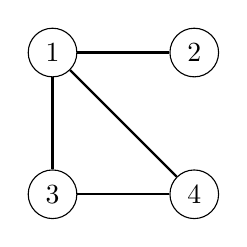
\begin{tikzpicture}[scale=0.9]
\node[draw, circle] (1) at (1,3) {$1$};
\node[draw, circle] (2) at (3,3) {$2$};
\node[draw, circle] (3) at (1,1) {$3$};
\node[draw, circle] (4) at (3,1) {$4$};

\path[draw,thick,-] (1) -- (2);
\path[draw,thick,-] (1) -- (3);
\path[draw,thick,-] (3) -- (4);
\path[draw,thick,-] (1) -- (4);
\end{tikzpicture}
\end{center}
té tres arbres d'expansió:
\begin{center}
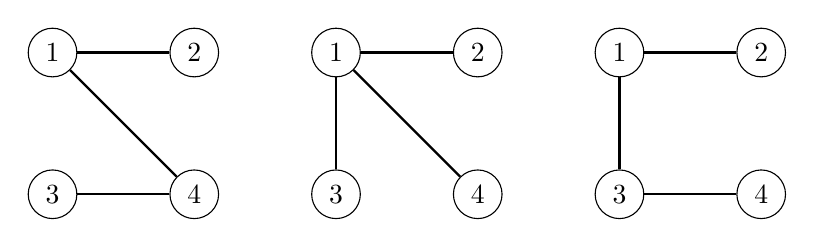
\begin{tikzpicture}[scale=0.9]
\node[draw, circle] (1a) at (1,3) {$1$};
\node[draw, circle] (2a) at (3,3) {$2$};
\node[draw, circle] (3a) at (1,1) {$3$};
\node[draw, circle] (4a) at (3,1) {$4$};

\path[draw,thick,-] (1a) -- (2a);
%\path[draw,thick,-] (1a) -- (3a);
\path[draw,thick,-] (3a) -- (4a);
\path[draw,thick,-] (1a) -- (4a);

\node[draw, circle] (1b) at (1+4,3) {$1$};
\node[draw, circle] (2b) at (3+4,3) {$2$};
\node[draw, circle] (3b) at (1+4,1) {$3$};
\node[draw, circle] (4b) at (3+4,1) {$4$};

\path[draw,thick,-] (1b) -- (2b);
\path[draw,thick,-] (1b) -- (3b);
%\path[draw,thick,-] (3b) -- (4b);
\path[draw,thick,-] (1b) -- (4b);

\node[draw, circle] (1c) at (1+8,3) {$1$};
\node[draw, circle] (2c) at (3+8,3) {$2$};
\node[draw, circle] (3c) at (1+8,1) {$3$};
\node[draw, circle] (4c) at (3+8,1) {$4$};

\path[draw,thick,-] (1c) -- (2c);
\path[draw,thick,-] (1c) -- (3c);
\path[draw,thick,-] (3c) -- (4c);
%\path[draw,thick,-] (1c) -- (4c);
\end{tikzpicture}
\end{center}
\index{Matriu Laplaciana} Per calcular el nombre d'arbres d'expansió,
construïm una \key{matriu Laplaciana} $L$, on $L[i,i]$ és el grau del
node $i$ i $L[i, j]$ és $-1$ si hi ha una aresta entre els nodes $i$ i $j$,
i $0$. La matriu Laplaciana del graf anterior és la següent:
\[
L= \begin{bmatrix}
  3 & -1 & -1 & -1 \\
  -1 & 1 & 0 & 0 \\
  -1 & 0 & 2 & -1 \\
  -1 & 0 & -1 & 2 \\
 \end{bmatrix}
\]


Es pot demostrar que el nombre d'arbres d'expansió és igual al
determinant de la matriu que s'obté quan eliminem qualsevol fila i
qualsevol columna de $L$. Per exemple, si eliminem la primera fila i
columna, el resultat és
\[
\begin{bmatrix}
  1 & 0 & 0 \\
  0 & 2 & -1 \\
  0 & -1 & 2 \\
 \end{bmatrix}
) =3.\]

El determinant és sempre el mateix, sense importar quina fila i columna eliminem
de $L$.

La fórmula de Cayley del capítol~\ref{cayley-formula} és un
cas especial del teorema de Kirchoff, ja que en un graf complet
de $n$ nodes es compleix

\[ \det(
\begin{bmatrix}
  n-1 & -1 & \cdots & -1 \\
  -1 & n-1 & \cdots & -1 \\
  \vdots & \vdots & \ddots & \vdots \\
  -1 & -1 & \cdots & n-1 \\
 \end{bmatrix}
) =n^{n-2}.\]
